\begin{figure}[!ht]
  \centering
  % Accuracy on test set: 11.41%, loss 2.86
  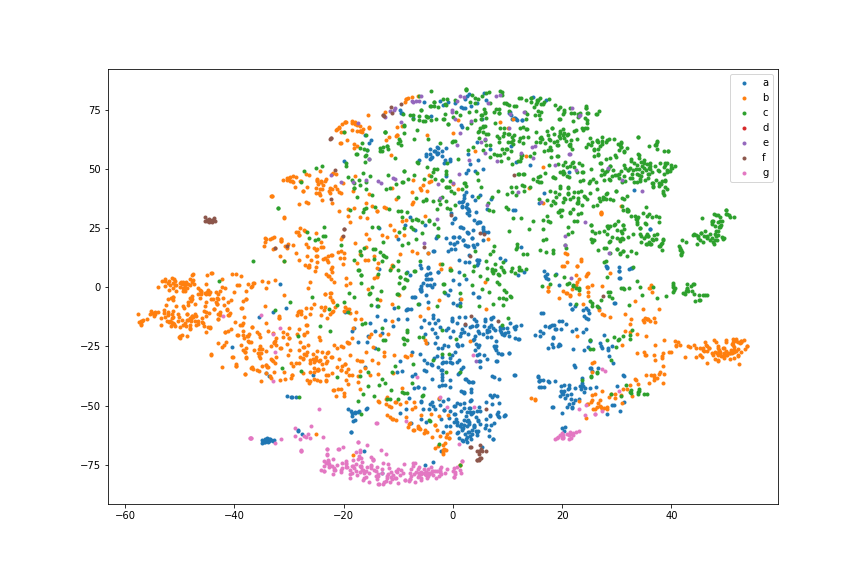
\includegraphics[width=0.33\linewidth]{latex/imgs/tsne_1_layer_with_schedule_256_final.png}
  % Accuracy on test set: 12.43%, loss 2.84
  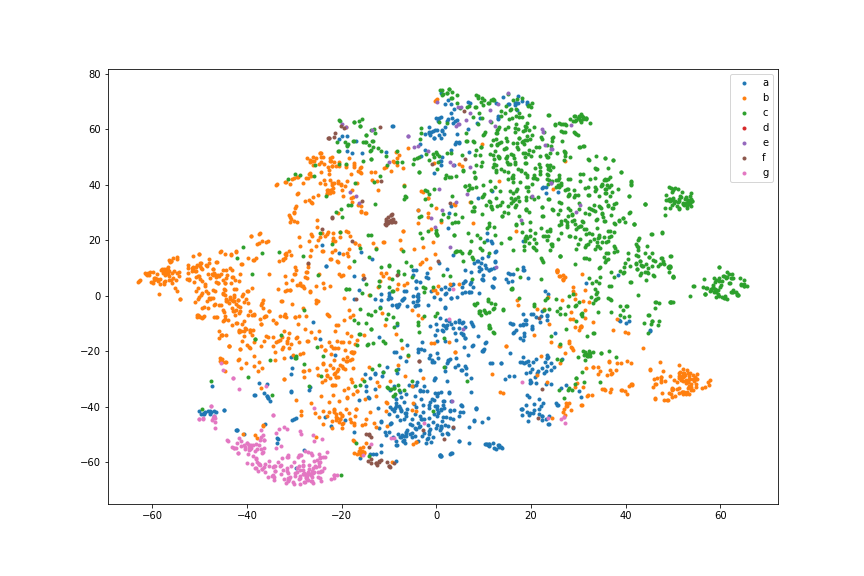
\includegraphics[width=0.33\linewidth]{latex/imgs/tsne_1_layer_with_schedule_512_final.png}
  % Accuracy on test set: 14.37%, loss 2.79
  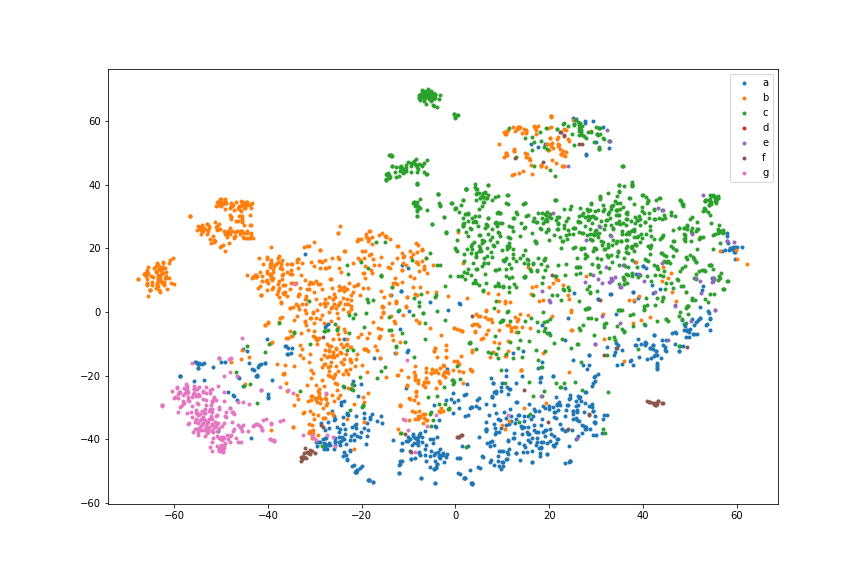
\includegraphics[width=0.33\linewidth]{latex/imgs/tsne_1_layer_with_schedule_1024_final.png}

  % 0.435 and 0.424
  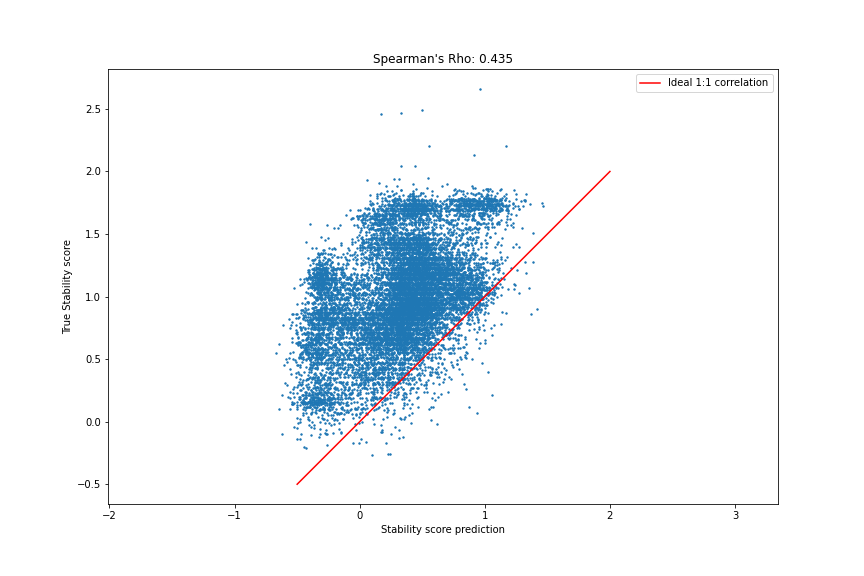
\includegraphics[width=0.33\linewidth]{latex/imgs/spearman_1_layer_with_schedule_256_final.png}
  % 0.428 and 0.414
  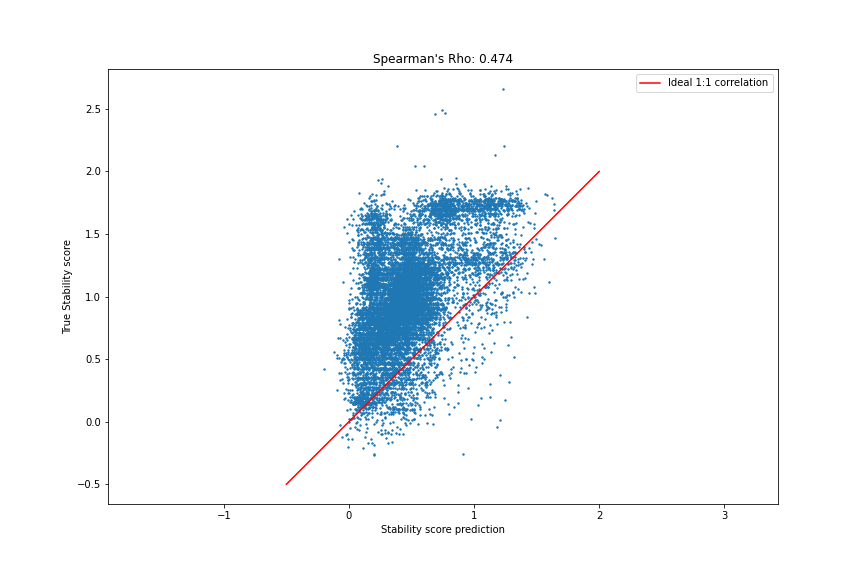
\includegraphics[width=0.33\linewidth]{latex/imgs/spearman_1_layer_with_schedule_512_final.png}
  % 0.507 and 0.627
  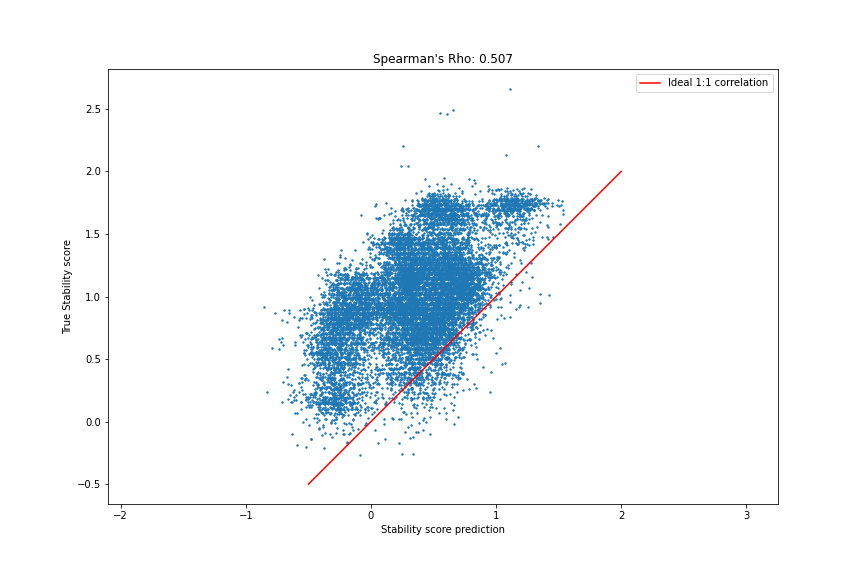
\includegraphics[width=0.33\linewidth]{latex/imgs/spearman_1_layer_with_schedule_1024_final.png}
  \caption{TSNE dimensionality reduction  and Spearman's rho data plots of the two models. Left is $256$ features, middle is $512$ features, right is $1024$ features.}
\end{figure}

\begin{table}[!ht]
\begin{tabular}{|l|l|l|l|l|}
\hline
              & Epochs trained & Next token prediction accuracy & Test Loss & Spearman's rho\\ \hline
256 features  & 60             & 11.41\%                        & 2.86      & 0.435         \\ \hline
512 features  & 30             & 12.43\%                        & 2.84      & 0.428         \\ \hline
1024 features & 10             & 14.37\%                        & 2.79      & 0.507         \\ \hline
\end{tabular}
\end{table}